\newglossaryentry{bigdata}
{
  name={big data},
  description={is a buzzword term primarily referring to data exceeding volume and size so that it cannot be properly handled with more traditional approaches and technologies anymore}
}


In this appendix, design\index{design} and architecture\index{architecture} of the software prototype\index{prototype} is presented.
First of all, a general overview of the system is given.
Followed by more in-depth dives into various parts and components of the solution.
Moreover, technical foundations of the implementation are described and their interplay explained.


\subsection{System Overview}

The prototypically\index{prototype} implemented, proposed solution is basically a web application.
It can be run locally as well as deployed to a hosted server environment.
This hosting is possible to be conveniently performed via \emph{Docker}\footnote{\textcolor{blue}{\href{https://www.docker.com/what-docker}{www.docker.com/what-docker}}} containerization.
The system consists of a web frontend and an \textsc{API} backend.
Both of which can be hosted as separate Docker containers.
The application is targeting and, hence, optimized for desktop browser clients.
So, the frontend mainly emits \textsc{HTML}/\textsc{CSS}/\textsc{JS} and communicates with its respective client via \textsc{HTTP(S)}.

The frontend is a \emph{Node.js}\footnote{\textcolor{blue}{\href{https://nodejs.org/en/about/}{nodejs.org/en/about/}}} application and the backend a \emph{\gls{jvm}} one.
On the frontend, the \gls{ui} is (pre-)rendered server-side in addition to client-side.
This technique is called isomorphic or universal rendering.
On the backend, data is stored and queried via \emph{Elasticsearch}\footnote{\textcolor{blue}{\href{https://www.elastic.co/products/elasticsearch}{www.elastic.co/products/elasticsearch}}}, a high-performance search and real-time analytics engine as well as document store, while transformed\index{transformation} and analyzed via \emph{Apache Spark}\footnote{\textcolor{blue}{\href{https://spark.apache.org/}{spark.apache.org}}}.

The latter is an engine for large-scale, near real-time data processing with convenient access to \gls{ml} algorithms via its \emph{MLlib} extension library.
Communication between backend and frontend is conducted with \gls{rest}, cf. \cite{Fielding2000}, and WebSockets\footnote{\textcolor{blue}{\href{https://tools.ietf.org/html/rfc6455}{tools.ietf.org/html/rfc6455}}}.
Figure~\ref{fig:system-overview} is presenting this system overview from a bird's eye view.


\subsubsection{In a Nutshell}

\begin{figure}[h]
  \centering
  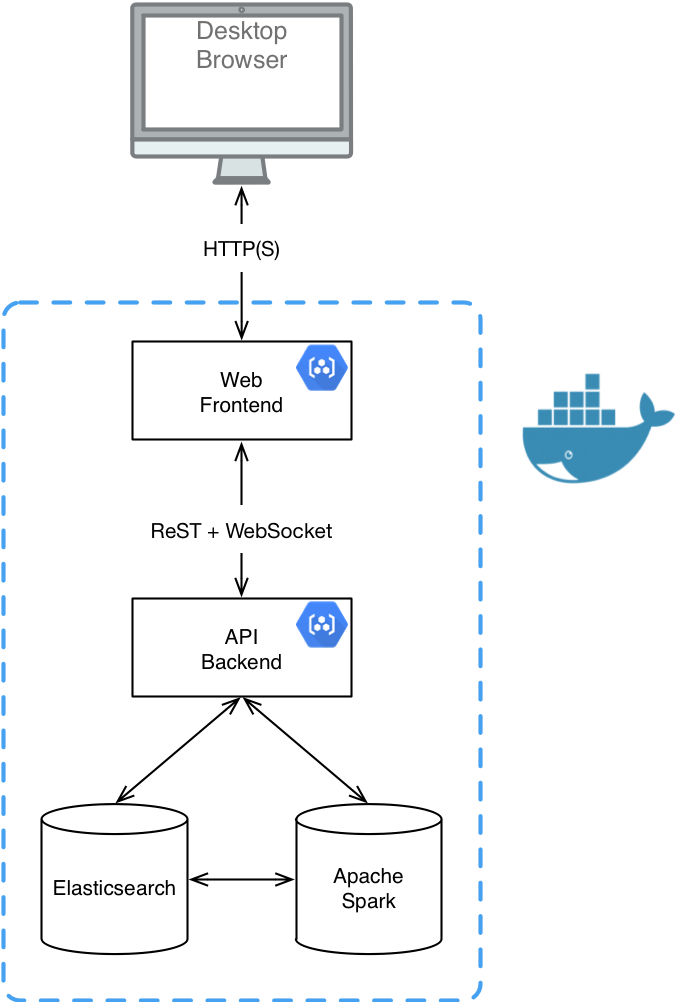
\includegraphics[width=0.75\textwidth]{figures/architecture/system-overview}
  \caption{High-level diagram of our SW architecture.}
  \label{fig:system-overview}
\end{figure}
\index{architecture}

\subsubsection{Going Live with Docker}

As mentioned above, the system is basically ``dockerized'' for container-based hosting.
I.e., the frontend as well as backend are each equipped with a fitting \emph{Dockerfile}.
Container images are based on the lightweight \emph{Alpine Linux}\footnote{\textcolor{blue}{\href{https://www.alpinelinux.org/about/}{www.alpinelinux.org/about/}}} distribution which is particularly well suited for that purpose.
In order to support an agile development process, it is easy to build and deploy the application.
More concretely, there is a \emph{Makefile} set up which allows for quick deployment of Docker images (incl. building and publishing these via private Docker repositories) to a virtual host.
The author chose in this example \emph{DigitalOcean}\footnote{\textcolor{blue}{\href{https://www.digitalocean.com/}{www.digitalocean.com}}} as hosting service provider due to the convenient \emph{\gls{dx}} it offers.

Multiple host nodes as well as multiple instances of either backend or frontend container were not relevant for the purpose of this prototype\index{prototype}.
It is generally possible to set this up and basically supported, though.
Moreover, Elasticsearch and Spark are simply being run in embedded mode within the backend component.
Again, it is generally possible to configure connection to real dedicated clusters of each.
Yet, the point of this prototype\index{prototype} was not really geared towards proving \emph{``\gls{bigdata}''} load capabilities.

On the virtual host an \emph{Nginx}\footnote{\textcolor{blue}{\href{https://nginx.org/en/}{nginx.org/en/}}} web server is configured to proxy the local containerized application servers to the public Internet.
Access to the web application is then restricted via \textsc{HTTP} basic authentication.
\textsc{HTTPS} is enabled through \emph{Let's Encrypt}\footnote{\textcolor{blue}{\href{https://letsencrypt.org/about/}{letsencrypt.org/about/}}}. \\
The interested reader may ask the author for a link with credentials.

\subsubsection{Project Structure and Setup}

In general, the system is comprised of three software projects.
One for the backend application, one for the frontend, and sort of an ``umbrella'', the master one.
The latter pulls the former ones in, via \emph{Git} submodule setup.
So, Git is used as \gls{vcs}, respectively for \gls{scm} with private \emph{Github} repositories, owned by the developer.
\gls{fs} structure of this master one also loosely resembles \emph{\glslink{cvast}{CVAST}} research group guidelines\footnote{\textcolor{blue}{\href{http://www.cvast.tuwien.ac.at/node/27}{www.cvast.tuwien.ac.at/node/27}}}.
Furthermore, it contains aforementioned Makefile for convenient builds and deployments.
The \gls{ci} tooling of choice is \emph{CircleCI}\footnote{\textcolor{blue}{\href{https://circleci.com/}{circleci.com}}}, a \gls{saas} provider with a good \gls{dx}.
Build tool of the backend project is \emph{Gradle}\footnote{\textcolor{blue}{\href{https://gradle.org/}{gradle.org}}}.
The frontend uses a combination of \emph{Yarn}\footnote{\textcolor{blue}{\href{https://yarnpkg.com/en/}{yarnpkg.com/en/}}} dependency management and \emph{Gulp}\footnote{\textcolor{blue}{\href{http://gulpjs.com/}{gulpjs.com}}} task scripts. Source code documentation is generated with \emph{Dokka}\footnote{\textcolor{blue}{\href{https://kotlinlang.org/docs/reference/kotlin-doc.html}{kotlinlang.org/docs/reference/kotlin-doc.html}}} for the backend, and \emph{ESDoc}\footnote{\textcolor{blue}{\href{https://esdoc.org/}{esdoc.org}}} for the frontend.


\subsection{Backend}

The backend mainly consists of the high-level components as laid out in Figure~\ref{fig:backend-components}.
It is basically a \emph{Spring\footnote{\textcolor{blue}{\href{projects.spring.io/spring-framework/}{projects.spring.io/spring-framework/}}} Boot\footnote{\textcolor{blue}{\href{https://projects.spring.io/spring-boot/}{projects.spring.io/spring-boot/}}}} application using \emph{Spring MVC} for its \gls{rest} controller layer.
\emph{Spring Messaging} is used for transparent WebSocket communication, and \emph{Reactor\footnote{\textcolor{blue}{\href{https://projectreactor.io/}{projectreactor.io}}} Event Bus} for reactive messaging within the outlier detection implementation.
The Elasticsearch data layer is based on \emph{Spring Data Elasticsearch\footnote{\textcolor{blue}{\href{http://projects.spring.io/spring-data-elasticsearch/}{projects.spring.io/spring-data-elasticsearch/}}}}.
Connection between Elasticsearch data storage and Apache Spark processing is done via \emph{ES-Hadoop} connector libraries\footnote{\textcolor{blue}{\href{https://www.elastic.co/guide/en/elasticsearch/hadoop/current/spark.html}{www.elastic.co/guide/en/elasticsearch/hadoop/current/spark.html}}}.

\begin{figure}[h]
  \centering
  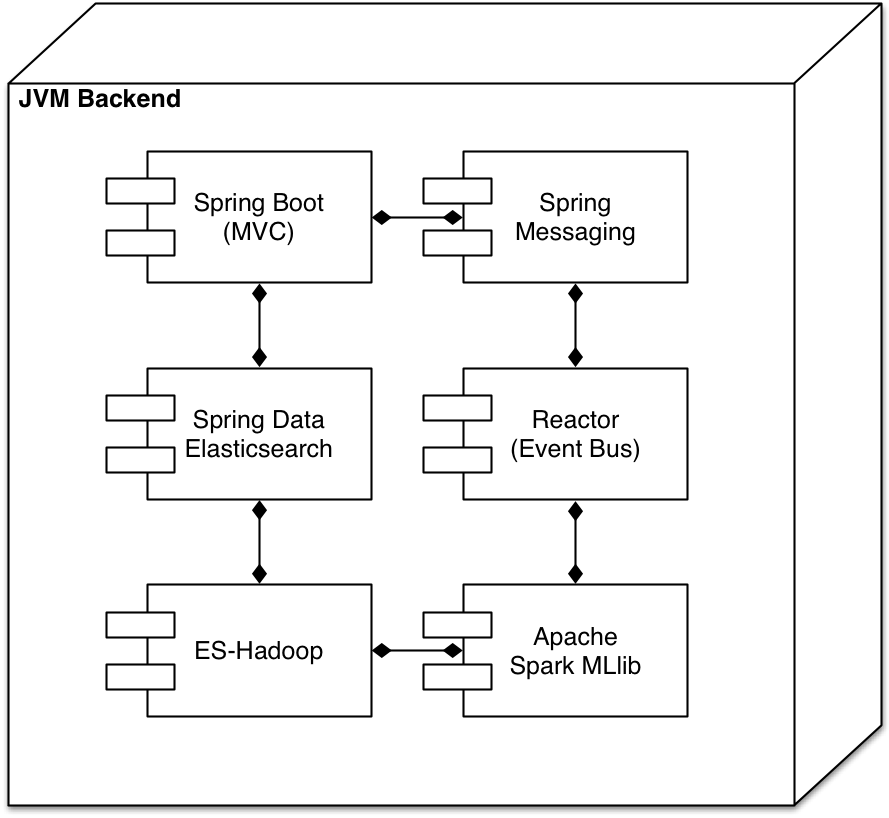
\includegraphics[width=0.75\textwidth]{figures/architecture/backend-components}
  \caption{Backend components diagram.}
  \label{fig:backend-components}
\end{figure}

Documentation of the \gls{rest} \textsc{API} is generated via \emph{Spring REST Docs\footnote{\textcolor{blue}{\href{https://projects.spring.io/spring-restdocs/}{projects.spring.io/spring-restdocs/}}}}.
This integrates nicely into the automated testing infrastructure of the project.
Thus, it can be seen as a superior solution compared to the en-vogue \emph{Swagger\footnote{\textcolor{blue}{\href{http://swagger.io/}{swagger.io}}}} in respect of it is possible to combine automated documentation generation with manually written one via
\emph{Asciidoctor\footnote{\textcolor{blue}{\href{http://asciidoctor.org/}{asciidoctor.org}}}}.

The backend project itself prefers structuring its top-level packages semantically.
E.g., there is a top-level package \emph{\textbf{importexport}} containing \emph{\textbf{dao}} (as in \emph{Data Access Object}) and \emph{\textbf{service}} sub-level packages -- not the other way round, as it would be more traditional fashion.
Unit and integration tests are present, written with state-of-the-art libraries.

Some deeper dive into the technologies employed for the backend follows.


\subsubsection{Kotlin on the JVM}

The \emph{Kotlin}\footnote{\textcolor{blue}{\href{https://kotlinlang.org/}{kotlinlang.org}}} programming language, by \emph{JetBrains}, is used on the backend.

It is a relatively young, statically typed, and concise \gls{jvm}-based language with seamless Java interoperability.
Mainly, it is adding quite some syntactic sugar, reasonably, as well as increased type inference support.
Plus, it is resolving some of Java's pain points, such as reference nullability -- a.k.a. the \emph{``billion-dollar mistake''\footnote{\textcolor{blue}{\href{http://lambda-the-ultimate.org/node/3186}{lambda-the-ultimate.org/node/3186}}}}.
Generally, it is taking a pragmatic stance and focuses on industrial software development needs.
As opposed to, e.g., Scala which can be seen as quite similar in various aspects, while being more computer science and particularly research focused, though.

Figure~\ref{fig:kotlin-sample} shows an exemplary code snippet.

\begin{figure}[h]
  \centering
  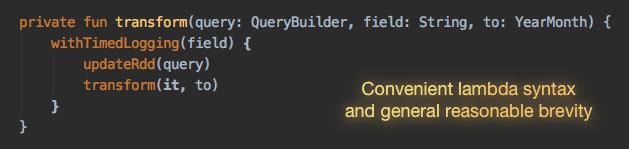
\includegraphics[width=1.0\textwidth]{figures/architecture/kotlin-sample}
  \caption{Kotlin sample demonstrating some of its useful features.}
  \label{fig:kotlin-sample}
\end{figure}

\subsubsection{Microservices with Spring Boot}

Spring Boot offers a useful approach\index{approach} to developing and running microservices. \\
It was, originally, heavily inspired by the \emph{Dropwizard}\footnote{\textcolor{blue}{\href{http://www.dropwizard.io/}{www.dropwizard.io}}} project.

The topic of building microservices itself is covered well in \cite{Newman2015}.
The basic idea here is to develop small, self-contained, and purpose-focused services with corresponding monitoring, provisioning, and orchestration capabilities.
This stands in rather stark contrast to the more traditional approach\index{approach} of building monolithic applications.
So, in general, Spring Boot provides a lot of features and abstractions with little necessary configuration out-of-the-box.
Furthermore, it integrates well with Kotlin, both sharing a pragmatic paradigm of software development philosophy.

\subsubsection{From Elasticsearch to ES-Hadoop} \label{sec:es-hadoop}

At the heart of data storage and querying, Elasticsearch is in use. \\
Spring Data Elasticsearch is providing some convenient abstractions.

As mentioned above, data processing, i.e., transformation\index{transformation} operations and outlier detection, is performed via Apache Spark and its MLlib.
Native bridging of these two popular \gls{bigdata} technologies is provided via ES-Hadoop connector libraries.
This is, basically, rooted in the fact that Apache Spark was born within the Apache Hadoop\footnote{\textcolor{blue}{\href{https://hadoop.apache.org/}{hadoop.apache.org}}} ecosystem.
Spark can be run completely independent from Hadoop infrastructure, though.
The connector libraries are officially supported and developed by \emph{Elastic\footnote{\textcolor{blue}{\href{https://www.elastic.co/}{www.elastic.co}}}}, the company behind Elasticsearch and related products.
In addition to the Scala \textsc{API}, since Spark is written in Scala, a Java \textsc{API} is available which is used in our project.

\subsubsection{Apache Spark \& MLlib}

As aforementioned, Spark is at the heart of data processing.

Its foundational construct is called \emph{\gls{rdd}}.
That is, the main concept is to provide a scalable solution for loading large datasets into memory, utilizing distributed computing.
One then can easily perform transformational\index{transformation} operations, like the common functional \emph{map} routine, on such an \gls{rdd}.
The underlying complexities are transparently hidden beneath by the abstraction.
This can be seen as fitting nicely into the philosophy of \emph{``\textbf{simple made easy}''}, as advocated by \emph{Rich Hickey}\footnote{\textcolor{blue}{\href{https://www.infoq.com/presentations/Simple-Made-Easy}{www.infoq.com/presentations/Simple-Made-Easy}}}.

Additionally, extension libraries have been built enhancing processing capabilities.
One of them is MLlib which provides convenient access to \gls{ml} algorithms.
This is used in our project for its temporal outlier detection implementation.

\subsubsection{Reactive Messaging}

Reactive programming is rather popular these days. \\
At its core stands the so-called \emph{Reactive Manifesto}\footnote{\textcolor{blue}{\href{http://www.reactivemanifesto.org/}{www.reactivemanifesto.org}}}.

It is a term for event-based programming.
That is, publish/subscribe mechanisms for message-driven communication.
Historically, it is build upon the notions from the classic \emph{Observer} pattern enhanced with functional programming techniques.
This paradigm fits especially well with the requirement of asynchronous notifications for the outlier detection component of our system. \\
Consequently, it is employed therein.

Concrete library used is Reactor and its implementation of the \emph{Event Bus} abstraction.
The former is, generally, a modern high-level take on the \emph{ReactiveX}\footnote{\textcolor{blue}{\href{http://reactivex.io/}{reactivex.io}}} approach\index{approach}.


\subsection{Frontend}

The frontend is a modern Node.js application. It is based on \emph{Este.js}\footnote{\textcolor{blue}{\href{https://github.com/este/este}{github.com/este/este}}}, a useful assembly of libraries and best practices for easily bootstrapping a universal \emph{Redux/React} project.

Its further refined stack for our project, basically, comprises of \emph{Isomorphic Fetch}\footnote{\textcolor{blue}{\href{https://github.github.io/fetch/}{github.github.io/fetch/}}} for \gls{rest} layer communication, \emph{STOMP over WebSocket}\footnote{\textcolor{blue}{\href{http://jmesnil.net/stomp-websocket/doc/}{jmesnil.net/stomp-websocket/doc/}}} with \emph{SockJS}\footnote{\textcolor{blue}{\href{http://sockjs.org/}{sockjs.org}}} for communicating with the corresponding Spring Messaging interface on the backend, a Redux\footnote{\textcolor{blue}{\href{http://redux.js.org/}{redux.js.org}}} layer containing business logic, a React\footnote{\textcolor{blue}{\href{https://facebook.github.io/react/}{facebook.github.io/react/}}} \gls{ui} as well as related URL path routing, plus \gls{ui} toolkits including \emph{D3.js}\footnote{\textcolor{blue}{\href{https://d3js.org/}{d3js.org}}} charting or common respectively extensible \gls{ui} components, and all running on an \emph{Express}\footnote{\textcolor{blue}{\href{http://expressjs.com/}{expressjs.com}}} web framework based server (see Figure~\ref{fig:frontend-components}).

\begin{figure}[h]
  \centering
  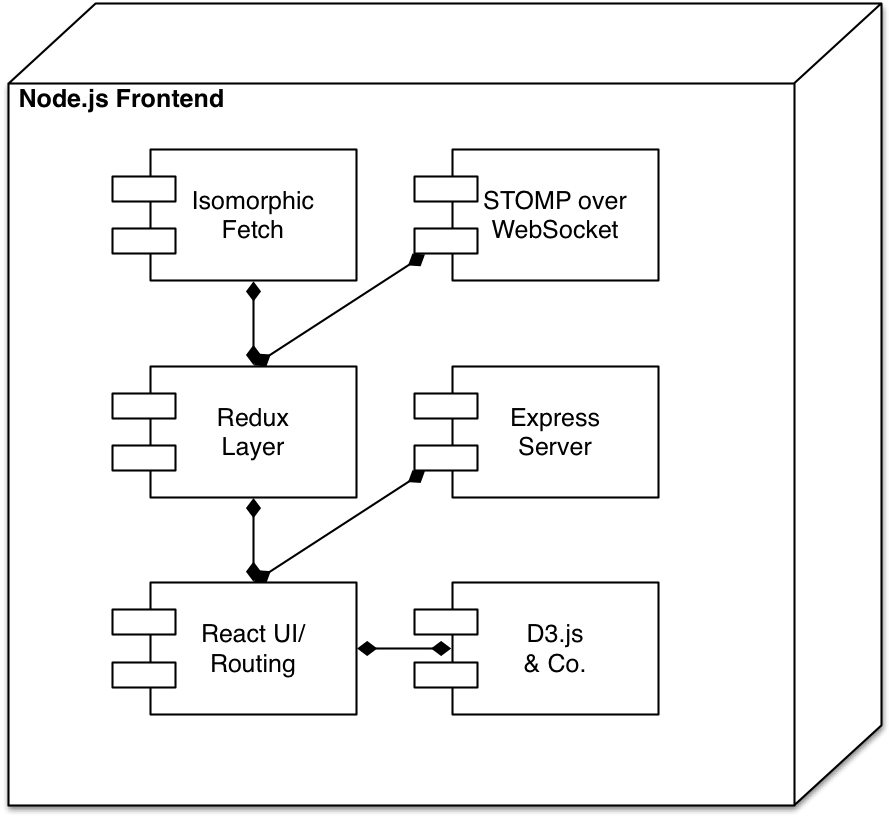
\includegraphics[width=0.75\textwidth]{figures/architecture/frontend-components}
  \caption{Frontend components diagram.}
  \label{fig:frontend-components}
\end{figure}

Project structure outlines an adapted Este scaffold. Automated testing is based on \emph{Jest}\footnote{\textcolor{blue}{\href{https://facebook.github.io/jest/}{facebook.github.io/jest/}}}.


\subsubsection{Contemporary JavaScript}

The frontend application is written in contemporary JS, that is, \emph{flow-typed\footnote{\textcolor{blue}{\href{https://flowtype.org/}{flowtype.org}}} ES6+}.

Figure~\ref{fig:react-flow-sample} is demonstrating some useful features as well as techniques when used together with Redux/React. Static type-checking is especially valuable for detecting bugs and errors early, at compile time. Compilation to common ES5 is performed via \emph{Babel}\footnote{\textcolor{blue}{\href{https://babeljs.io/}{babeljs.io}}} plus a \emph{Webpack}\footnote{\textcolor{blue}{\href{https://webpack.js.org/}{webpack.js.org}}} toolchain is in place -- minifying, optimizing, and bundling web app assets.
In addition, \emph{ESLint\footnote{\textcolor{blue}{\href{http://eslint.org/}{eslint.org}}}} helps keeping the code clean and adhering to good practices.

\subsubsection{React with Material Design}

As mentioned, the \gls{ui} is based on React.
A technology and library created at \emph{Facebook Engineering}.
It enables one to build composable \gls{ui} components in a declarative way, clearly reasoning about their state via cleanly applied \emph{\gls{soc}} pattern.
Templating is achieved with so-called \emph{JSX\footnote{\textcolor{blue}{\href{https://facebook.github.io/react/docs/introducing-jsx.html}{facebook.github.io/react/docs/introducing-jsx.html}}}}.
That is, \textsc{XML}-like syntax embedded directly in \textsc{JS} code.
Moreover, its performance is really good as partial re-rendering of to-be-updated \gls{dom} tree nodes is supported transparently.

The React programming model usually takes a bit to get accustomed to, but its benefits do pay off, especially in the long run.
Particularly, clear separation of application state and \gls{dom} is a big leap forward in this space.

General \gls{ux} of the \gls{ui} of our application is based on the \emph{Material Design\index{design}}\footnote{\textcolor{blue}{\href{https://material.io/}{material.io}}} approach\index{approach} and specification by Google.
As implementing components kit, \emph{React Toolbox}\footnote{\textcolor{blue}{\href{http://react-toolbox.com/}{react-toolbox.com}}} is used. It provides a quite comprehensive, carefully crafted set of common \gls{ui} controls and elements.
For \textsc{CSS} needs, transpiled \emph{Sass\footnote{\textcolor{blue}{\href{http://sass-lang.com/}{sass-lang.com}}}} is employed, which is pretty popular for this use case.

As mentioned before, the application is rendered client-side, as commonly expected from a \gls{spa}, yet, initially also server-side.
This isomorphic pre-rendering on the server improves the \gls{ux} by minimizing potential, irritating ``flicker'' effects on initial page load.
In particular, when loading a page with an URL which requires routing.
Additionally, it helps with \gls{seo} if applicable.
Routing is built on client \emph{HTML5 History API}\footnote{\textcolor{blue}{\href{http://diveintohtml5.info/history.html}{diveintohtml5.info/history.html}}} for clean, universal URL path layout.

\subsubsection{From Flux to Redux}

The \emph{Flux} architecture\index{architecture} was introduced by Facebook Engineering as an approach\index{approach} to better structuring \gls{spa}s.
It is based on the idea of strictly one-way data flow and binding.

This makes it much simpler to reason about an \gls{ui} system, and therefore less error-prone.
The basic concepts are shown in Figure~\ref{fig:flux-architecture} which stems from official documentation material\footnote{\textcolor{blue}{\href{https://facebook.github.io/flux/docs/in-depth-overview.html\#structure-and-data-flow}{facebook.github.io/flux/docs/in-depth-overview.html\#structure-and-data-flow}}}.
So, generally, actions are triggering system state changes and, consequently, \gls{ui} updates in a unidirectional manner.
Redux took theses concepts and further simplified them, iterating upon in its implementation.
Solutions for handling asynchronous events, as they are common in \gls{spa}s, include injecting a promise middleware into Redux as well as extending it with reactive processing via \emph{redux-observable\footnote{\textcolor{blue}{\href{https://redux-observable.js.org/}{redux-observable.js.org}}}} plus \emph{RxJS\footnote{\textcolor{blue}{\href{http://reactivex.io/rxjs/}{reactivex.io/rxjs/}}}}.
Both approaches\index{approach} are used in the prototype\index{prototype} to varying degrees with an emphasis on the former one, to get a feel for them.
A real product would most probably rather focus on one of them then.
ES6+ \emph{async/await} is helpful for coding with promises sequentially, saving one from \emph{``callback hell''}.
Immutable data structures and collections provided by \emph{Immutable.js\footnote{\textcolor{blue}{\href{https://facebook.github.io/immutable-js/}{facebook.github.io/immutable-js/}}}} are also commonly used.
Plus, \emph{Ramda\footnote{\textcolor{blue}{\href{http://ramdajs.com/}{ramdajs.com}}}} fits in well as a functional programming utilities library.
Speaking of utility libraries in our project, ones centered on temporal data processing are \emph{date-fns\footnote{\textcolor{blue}{\href{https://www.npmjs.com/package/date-fns}{www.npmjs.com/package/date-fns}}}} and \emph{js-joda\footnote{\textcolor{blue}{\href{https://js-joda.github.io/js-joda/}{js-joda.github.io/js-joda/}}}} (a \emph{java.time}-compliant \textsc{JS} port).

\begin{figure}[h]
  \centering
  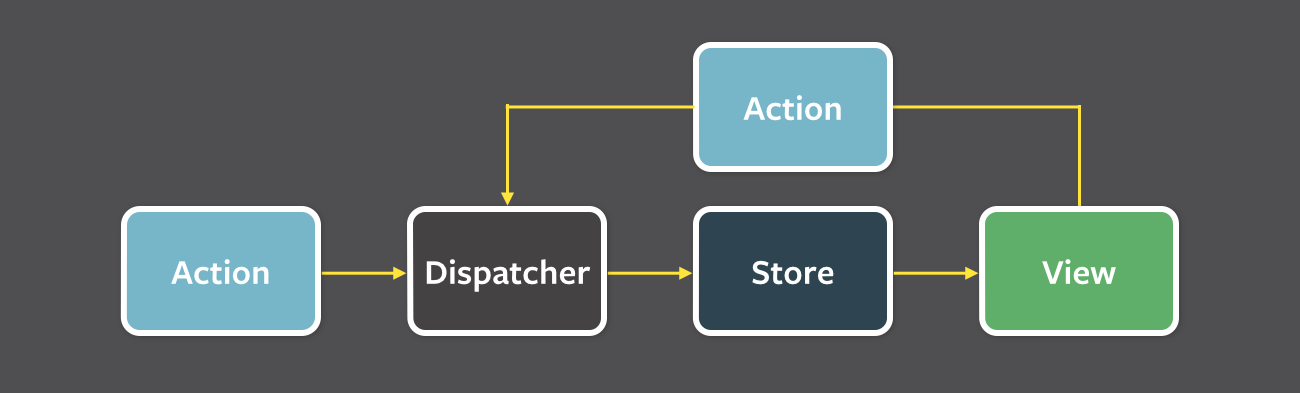
\includegraphics[width=1.0\textwidth]{figures/architecture/flux-simple}
  \caption{Simple Flux architecture diagram from Facebook Engineering.}
  \label{fig:flux-architecture}
\end{figure}
\index{architecture}

\subsubsection{Fetch API \& WebSockets}

The \emph{Fetch API} is a modern approach\index{approach} to \emph{Ajax} communication.
That is, asynchronous client/server communication of a browser application via \textsc{HTTP}.
This, traditionally, is based on usage of the so-called \emph{XMLHttpRequest} browser \textsc{JS} \textsc{API}.
The rather young Fetch \textsc{API} takes the basic concepts of async browser \gls{rest} calls and pours it into a contemporary form, conveniently usable.

\emph{WebSockets} allow for bidirectional communication.
That is, instead of solely pulling from a server, a browser client app is also able to get data pushed by the server.
It is especially useful in event-based systems, such as messaging-related ones.

\subsubsection{D3.js Charting}

\emph{D3.js} (as in \emph{Data-Driven Documents}) is a very popular \textsc{JS} library, primarily used for interactive charting.
Originally, it was developed at \emph{Stanford Vis Group} (see \cite{Bostock2011}).
It is based on \gls{svg} and surrounded by an ecosystem of components as well as extensions.

For most of the charts in our application, \emph{NVD3\footnote{\textcolor{blue}{\href{http://nvd3.org/}{nvd3.org}}}} is used.
It is a useful repository of various ready-to-use charts, all conveniently customizable.
Plus, they are nicely crafted with appealing default look \& feel, supporting decent animations.
Figure~\ref{fig:nvd3-gallery} shows an overview gallery from their documenting website.
Our calendar heatmap visualization component is based on \emph{cal-heatmap\footnote{\textcolor{blue}{\href{http://cal-heatmap.com/v2/}{cal-heatmap.com/v2/}}}}.
It is a widely used implementation with a multitude of customization and tweaking options.
Integration of D3 with React works, all in all, relatively straightforward. Yet, some resorting to direct \gls{dom} manipulation and event handling is required, unfortunately, due to legacy reasons inflicted by the former.

\begin{figure}[h]
  \centering
  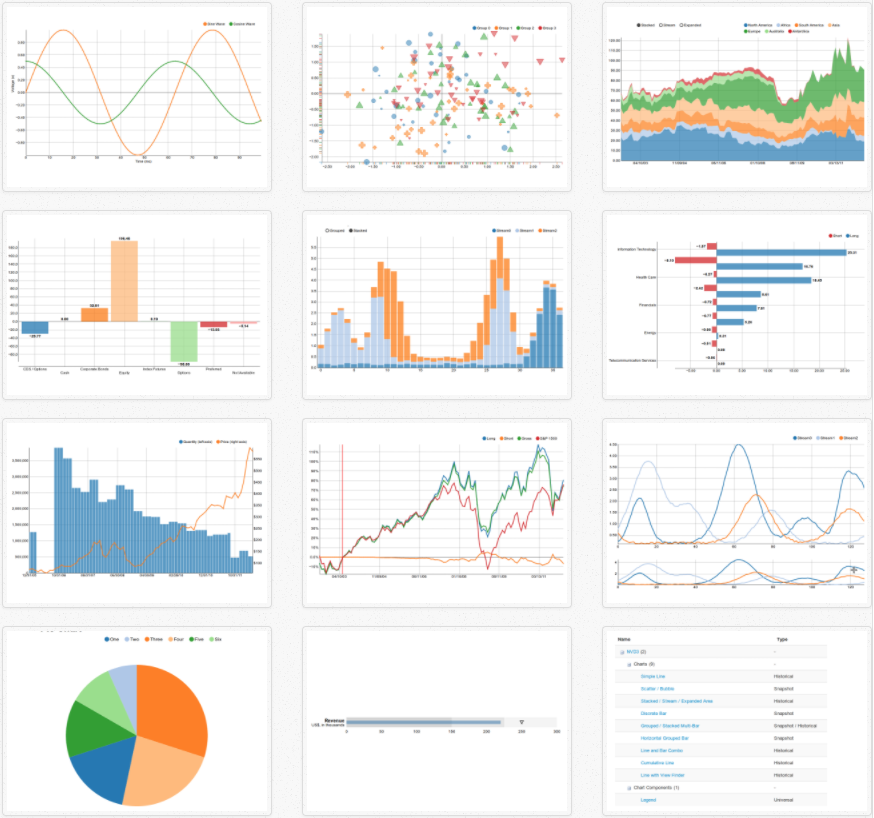
\includegraphics[width=0.825\textwidth]{figures/architecture/nvd3-gallery}
  \caption{A screenshot of an NVD3 charts gallery, as presented on nvd3.org.}
  \label{fig:nvd3-gallery}
\end{figure}

\begin{figure}[h]
  \centering
  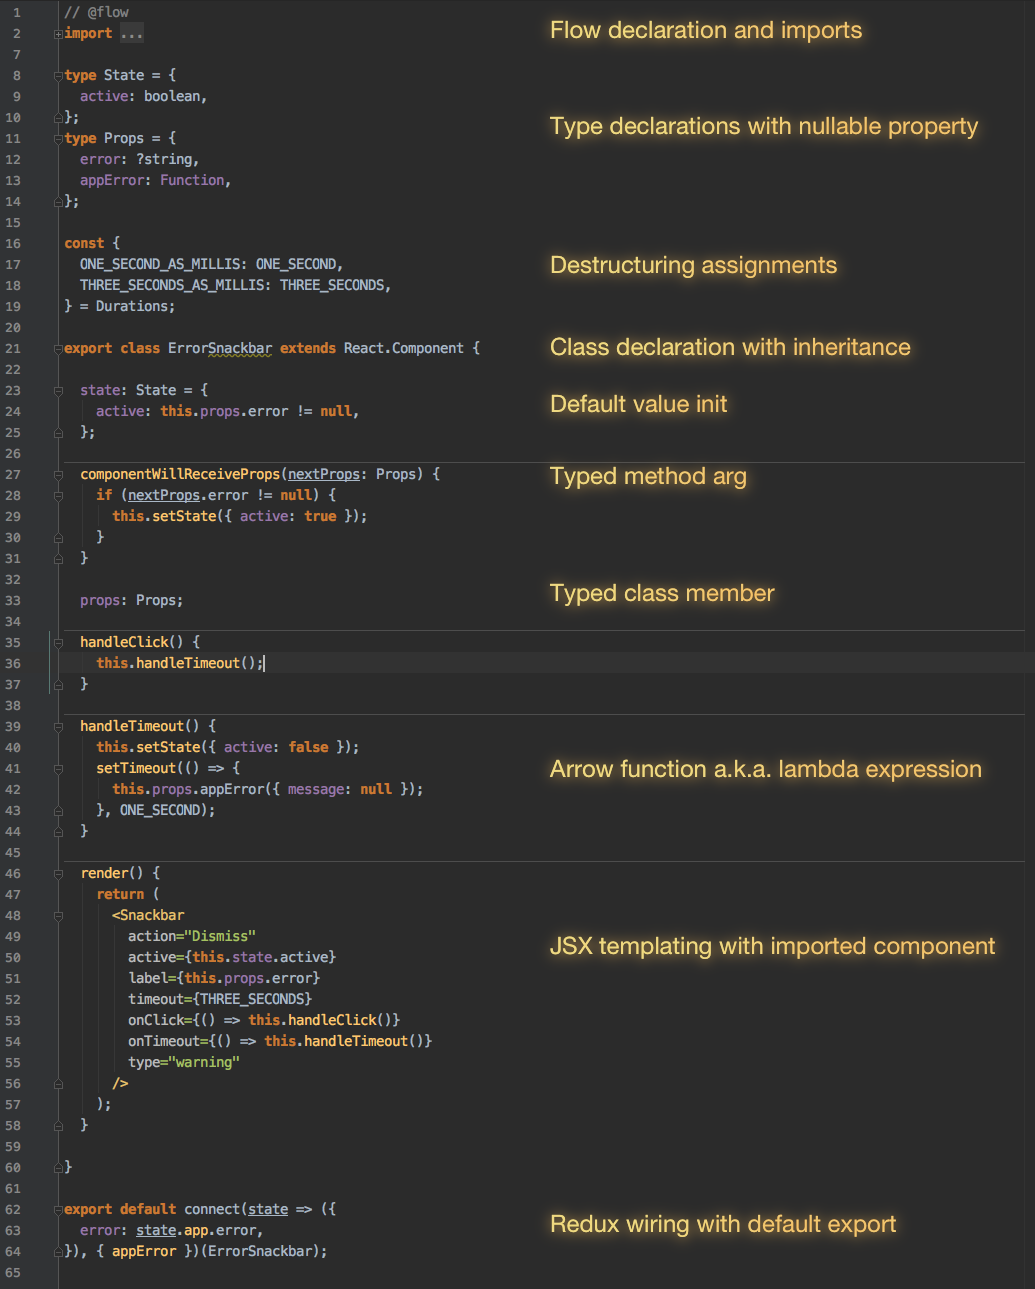
\includegraphics[width=1.05\textwidth]{figures/architecture/react-flow-sample}
  \caption{Flow-typed ES6+ Redux/React \gls{ui} component showing some useful features.}
  \label{fig:react-flow-sample}
\end{figure}
